

%!TEX root = /Users/sbogutzky/Entwicklung/projects/bogutzky/repositories/2939413/final-draft.tex
\section{Flow und Laufen (interindividuell)} 

% (fold)
\label{sec:flow_und_laufen_interindividuell}

\subsection{Einleitung} 

% (fold)
\label{sub:einleitung_5_3}

In Anbetracht der Erkenntnisse der ersten Laufstudie (Abschnitt~\ref{sub:diskussion_5_1}) gehen wir davon aus, das die Ebenen \emph{Physiologisch} und \emph{Motorisch} aus dem prozessorientierten Modell (Abbildung~\ref{fig:prozessorientiertes_flow_modell_2}) bei Flow-Zuständen in Zusammenhang stehen~\citep{Grueter2016a}. Dieser Zusammenhang drückt sich in Flow-Zuständen in einer individuellen optimalen Schrittfrequenz aus. Gleichzeitig steht die Schrittfrequenz mit der \ac{HR} und dem Bewegungsaufwand in Verbindung. Deshalb gehe ich davon aus, dass in der Regel niedrige individuelle optimale Herzschlagfrequenzen und eine niedrige individuelle optimale Bewegungsaufwände mit dem Flow-Erleben einhergehen, auch wenn ich dies in Abschnitt~\ref{sec:flow_und_laufen_intraindividuell} nicht belegen konnte. 

Alle drei genannten impliziten Merkmale konnten in der vorherigen Laufstudie keine prozessbasierten Erkenntnisse liefern. Die kardio-lokomotorische Phasensychronisation hingegen (Abschnitt~\ref{ssub:die_kardio_lokomotorische_phasensynchronisation}) kann diese Lücke schließen und stellt gleichzeitig die Verbindung der beiden Ebenen \emph{Physiologisch} und \emph{Motorisch} des prozessorientierten Modell (Abbildung~\ref{fig:prozessorientiertes_flow_modell_2} da. Zudem ist sie das einzige implizite Merkmale, welches unkompliziert bei interindividuellen Vergleichen einsetzbar ist. Die Vermutung das Flow-Erleben und hohe kardio-lokomotorische Phasensychronisation als zwei optimale Zustände beim Laufen direkt in Verbindung stehen konnte ich in der ersten Laufstudie nicht belegen (Abschnitt~\ref{sec:flow_und_laufen_intraindividuell}). Ich stellte die Vermutung an, dass es sich bei der kardio-motorischen Phasensynchronisation mit ihren drei Mustern (\emph{Schritt dominiert}, \emph{Gleichgewicht}, \emph{Herz dominiert}) um eine \emph{physiologisch messbare \ac{AFP}} handelt. Durch die Nutzung der kardio-motorischen Phasensynchronisation als Moderator sollte eine indirekte Verbindung zum Flow-Erleben nachweißbar sein. Im nachfolgenden Abschnitt beschreibe ich die Überprüfung dieser indirekte Verbindung und die Überprüfung des direkten positiven linearen Zusammenhang zwischen Flow-Erleben und der kardio-lokomotorischen Phasensychronisation. Die Untersuchung führte ich mit mehreren Untersuchungspersonen, die jeweils nur einmal liefen. Die Herangehensweise glich dem in Abschnitt~\ref{sec:herangehensweise} beschriebenen Herangehen: (1) Daten sammeln und Merkmale extrahieren, (2) Zusammenhänge zwischen expliziten und impliziten Merkmalen suchen und ggf. (3) den Prozess der Tätigkeit bzw. der Daten der Tätigkeit untersuchen. 

% subsection einleitung (end)
\subsection{Hypothesen} 

% (fold)
\label{sub:hypothesen}

Aus den in der Einleitung dargestellten Annahmen fasse ich die zwei nachfolgenden Forschungshypothesen für die beschriebene Studie zusammen: 
\begin{description}
	\item[$H^1$] Zwischen Flow-Erleben gemessen durch den Generalfaktor der \ac{FKS} und dem normalisierten Shannon Entropie Index der kardio-lokomotorischen Phasensynchronisation besteht ein positiver linearer Zusammenhang beim Laufen. 
	\item[$H^2$] Alternative: Zwischen den drei Mustern der kardio-lokomotorische Phasensynchronisation (\emph{Schritt dominiert}, \emph{Gleichgewicht}, \emph{Herz dominiert}) gibt es einen Unterschied zwischen \emph{Schritt dominiert} und \emph{Gleichgewicht} und eine Unterschied zwischen \emph{Gleichgewichtt} und \emph{Herz dominiert} im Bezug auf Flow-Erleben gemessen mit dem Generalfaktor der \ac{FKS}.
	
	%\item[$H^3$] Zwischen Flow-Erleben gemessen durch den Generalfaktor der \ac{FKS} und dem Bewegungsaufwand besteht ein negativer linearer Zusammenhang beim Laufen. 
\end{description}

% subsection hypothesen (end)
\subsection{Methode} 

% (fold)
\label{sub:methode_5_3}

An der Studie nahmen 36 gesunde männliche Untersuchungspersonen im Alter von 18 bis 40 Jahre ($M = 29; SD = 5{,}74$) teil. Zwanzig Untersuchungsteilnehmer gehörten der ersten Herrenmannschaft Fußball und zehn der Altherrenmannschaft Fußball des TSV Dörverden an. Zusätzlich liefen sechs Freizeitläufer in der Studie mit. Alle waren es gewohnt, mindestens eine halbe Stunde in der Woche zu laufen. Von den Untersuchungspersonen hatten vier schon an Laufereignissen wie Halbmarathon oder Marathon teilgenommen. Alle Untersuchungspersonen nahmen freiwillig ohne eine Vergütung an der Studie teil. 

Mit jeder Untersuchungsperson führte ich die Untersuchung einzeln durch. Die Untersuchung fand auf dem Sportplatzgelände, in den Kabinen des TSV Dörverden und auf einer naheliegenden Laufstrecke statt. Die einzelnen Untersuchungen führte ich im Zeitraum von Mitte März bis Ende Mai 2016 durch. Der Beginn jeder Sitzung variierte zwischen 16 Uhr und 19 Uhr und dauerte etwa eine Stunde. Jede Sitzung begann mit der persönlichen Begrüßung der Untersuchungsperson und mit dem Hinweis, dass ich als Untersuchungsleiter die Kommunikation vor dem Lauf möglichst gering halten möchte. Ich wies die Untersuchungspersonen daraufhin, dass sie sich im gesamten Verlauf der Sitzung in keiner Prüfungssituation befinden. Im Anschluss zog sich die Untersuchungsperson um und bereitete sich für etwa fünf Minuten auf den Lauf vor. 

Danach rüstete ich die Untersuchungsperson mit zwei Shimmer \acp{IMU} mit Gyro-Modulen am linken und rechten Unterschenkel unterhalb der Wade aus. Ich korrigierte die Trageposition der \acp{IMU} basiert auf übliche Tragepositionen auf Hinweisen aus der Literatur \citep[][]{Hreljac1993}. Durch die Identifikation beider Schritte im Bewegungsablauf des Laufens verspreche ich mir eine exaktere Berechnung der kardio-lokomotorischen Phasensynchronisation. Das Smartphone blieb wie in den beiden vorherigen Studien am Oberarm befestigt, diente aber nur als Datenverarbeitungsgerät. Es kam ein leistungsstarkes Sony Xperia Z1 mit Android Version 5.1.1 zum Einsatz.

Ich nutzte für die kardiovaskulären Messungen ein physiologisches Monitoring Modul namens BioHarness 3 des Unternehmens Zephyr. Das Modul gewährleistet durch eine interne Vorverarbeitung und eine Zwischenspeicherung gleichwertige kardiovaskuläre Messungen wie das Shimmer EKG-Modul. Vorteile des BioHarness 3 Moduls auf einem Brustgurt sind die einfachere Handhabung beim Anlegen und die Vorverarbeitung des \ac{EKG}-Signals durch das Modul selbst. Nach Herstellerangaben taste das Modul mit 1024~Hz ab. Das gesamte angelegte Equipment ist in Abbildung~\ref{fig:equipment_3} dargestellt. Die Untersuchungsperson wurde von mir angewiesen, jegliches technische Gerät und ggf. ihre Uhr während des Laufes abzulegen. 
\begin{figure}
	[!htb] \centering 
	\includegraphics[width=1.00 
	\textwidth]{equipment_3} \caption[Equipment der finalen Studie zum Flow-Erleben beim Laufen]{Equipment der finalen Studie zum Flow-Erleben beim Laufen.} \label{fig:equipment_3} 
\end{figure}

Die Laufstrecke wurde von mir ausgewählt (Abbildung~\ref{fig:landkarte_3}), da sie von allen Fußballern des TSV Dörverden des Öfteren gelaufen wurde. Alle Freizeitläufer kannten sich in Dörverden so weit aus, dass es für sie kein Problem war, die Laufstrecke ohne eine Karte zu laufen. Die Strecke besteht aus einem Rundkurs, den die Untersuchungsperson dreimal laufen musste. Die Gesamtstrecke betrug 4,5 Kilometer, war eben und die Untersuchungsperson lief auf Asphalt. Die Laufstrecke führt durch ein Waldgebiet mit geringem Verkehrsaufkommen. Sie besitzt eine merkbare Senkung, in der Regel sich ein Gefühl der Leichtigkeit einstellt. 
\begin{figure}
	[!htb] \centering 
	\includegraphics[height=0.50 
	\textheight]{landkarte_3} \caption[Laufstrecke -- Rundkurs]{Laufstrecke -- Rundkurs drei mal -- insgesamt 4,5~km (erstellt aus GPS-Positionen mit OpenStreetMap)} \label{fig:landkarte_3} 
\end{figure}

Ich erläuterte der Untersuchungsperson nach Zeigen der Laufstrecke, dass es in der Untersuchung nicht um die individuelle Laufleistung geht. Ich wies die Untersuchungsperson an, die Laufstrecke in einem Lauftempo zu laufen, das sich für die Untersuchungsperson optimal anfühlt, diese nicht überfordert oder unterfordert. Trotz dieser Anweisung ging ich von Ausreißern nach unten und nach oben aus, da bei jüngeren Fußballern öfters der direkte Vergleich mit anderen im Vordergrund steht und bei einigen der Gedanke vorherrscht, mit wenig Leistung das Optimum zu erreichen. 

Danach begleitete ich die Untersuchungsperson aus der Kabine und startete die Datenaufnahme am Smartphone über den \ac{PPC}. Direkt im Anschluss führte die Untersuchungsperson den Lauf durch. Die Untersuchungsteilnehmer benötigten für die Laufstrecke im Durchschnitt 25 Minuten und 26 Sekunden. 

Ich erwartete den Läufer am Sportgelände zurück und stoppte bei Ankunft die Datenaufnahme. Die Untersuchungsperson beantwortete im Anschluss an eine kurze Erholungspause die \ac{FKS} auf Grundlage des Laufes. Im Gegensatz zur ersten Laufstudie führte ich eine Instruktion ein, die den Läufer anwieß, die Aussagen der \ac{FKS} auf den gerade beendeten Lauf zu beziehen. Nach der Befragung füllte die Untersuchungsperson ein Konsensformular aus. Ich beendete die Sitzung und begleitete die Untersuchungsperson aus der Kabine. Ich teilte keinem Läufer vor Abschluss der Studie Ergebnisse wie z.~B. Laufzeit mit. 

\subsection{Apparat} 

% (fold)
\label{sub:apparat}

In der beschriebenen Laufstudie kam eine erweiterte Version des \ac{PPC}s zum Einsatz. Wir erweiterten den \ac{PPC} dahin, dass er Daten des BioHarness 3 über Bluetooth empfangen und im Android Dateisystem speichern kann. Für alle Sensoren, ob interne \ac{GPS}-Einheit, Shimmer \ac{IMU} oder BioHarness erhält der \ac{PPC} die Daten über einen Android Service. Ein Service kapselt Programmlogik, die das Android OS unabhängig von der App ausführen kann. Android OS ist in der Lage, Services automatisch neu zu starten. Es ist möglich, ihnen eine höhere Ausführungspriorität als der sichtbaren Activity (Teil der App mit dem der Benutzer interagiert) zuzuordnen. Der Service ermöglicht, unterschiedlichen sichtbaren Activities die ankommenden Daten zu visualisieren. Wir hielten dieses gerade für die \ac{EKG}-Daten für notwendig, da wir als Untersuchende damit die Anbringung der Elektroden am Oberkörper und die zuverlässige Übertragung der \ac{EKG}-Daten im Vorlauf der Untersuchung überprüfen können. 

Der BioHarness 3 ist ein kompaktes physiologisches Monitoring Modul, das die Erhebung von physiologischen Daten ermöglicht. Er nimmt im Gegensatz zu den Shimmer \acp{IMU} mit Basis-Firmware einige Datenverarbeitungsschritte vor. Damit erhält der \ac{PPC} vom BioHarness 3 vorverarbeitete Daten wie die mittlere \ac{HR}, RR-Intervalle, Atemfrequenz, Haltungswinkel, Beschleunigung und Körpertemperatur des Untersuchenden. Das BioHarness-Modul kann die Untersuchungsperson unterschiedlich tragen: mit einem Brustgurt, mit klebbaren Elektroden oder in einem Kompressionsshirt. Ich nutzte in der beschriebenen Studie den mitgelieferten Brustgurt. Bei der Messung der kardiovaskulären Daten macht sich der BioHarness die Eigenschaft des Aktionspotenzials zunutze, indem er mit der Hilfe des Brustgurts die Veränderung des Potenzials über Äquipotenziallinien misst. Der Brustgurt misst mittels befeuchtbaren Elektrodenfeldern, die mit der Körperoberfläche an zwei verschiedenen Stellen in Kontakt sind, die Potenzialdifferenz. Erreicht die Differenz ein Maximum, geht das Modul von einem Herzschlag aus. 

Wir veränderten zusätzlich die Interaktion mit dem Fragebogen. In der genutzten Version des \ac{PPC} startet der Fragebogen erst durch die Interaktion der Untersuchungsperson, damit der \ac{PPC} die genaue Startzeit, die Dauer und die Endzeit der Selbstauskunft erfassen kann. Dadurch ist eine nachträgliche Identifikation, die in den vorherigen Studien durchgeführt wurde, nicht mehr nötig. 

Die Sensorkonfiguration der beschriebenen Studie ist der Tabelle~\ref{tab:sensorkonfiguration_3} zu entnehmen. Ich musste keine Veränderungen an der \ac{PPP} durchführen. 
\begin{table}
	[!htb] \caption[Sensorkonfiguration der finalen Studie zum Flow-Erleben beim Laufen]{Sensorkonfiguration der finalen Studie zum Flow-Erleben beim Laufen} \label{tab:sensorkonfiguration_3} 
	\begin{tabularx}
		{ 
		\textwidth}{p{.30 
		\textwidth} p{.20 
		\textwidth} p{.50 
		\textwidth}} \toprule & Abtastrate & Betriebssicherer Messbereich \\
		\midrule BioHarness EKG & 1024~Hz & \\
		Beschleunigungsmesser & 56,7~Hz & 1,5~g \\
		Kreiselinstrument & 56,7~Hz & 500 $deg \cdot s^{-1}$ \\
		\bottomrule 
	\end{tabularx}
\end{table}

Die \ac{PPP} erweiterte ich durch eine Funktion, die in der Lage ist in der relativen Phase der kardio-lokomotorischen Phasensynchronisation in einem konkreten Zeitabschnitt aufsteigende Punkte und absteigende Punkte zu identifizieren. Dies ermöglicht mir in der Analyse die einzelnen Läufe automatisch in die drei Gruppen (\emph{Schritt dominiert}, \emph{Gleichgewicht}, \emph{Herz dominiert}) zu kategorisieren. 

% subsection apparat (end)
\subsection{Operationalisierung und gewonnene Daten} 

% (fold)
\label{sub:operationalisierung_und_gewonnene_daten_5_3}

Von den 36 gewonnenen Datenaufzeichnungen habe ich fünf aus folgenden Gründen entfernt:
\begin{itemize}
	
	\item Ein Teilnehmer hatte eine langwierige Verletzung und beklagten Schmerzen nach dem Lauf.
	
	\item Bei einen Teilnehmer versagte die Aufnahme mit dem Bioharness
	
	\item Drei Teilnehmer haben die Beantwortung der nicht ernstgenommen oder die Aussagen nicht verstanden.
\end{itemize}

Nach Entfernung dieser Aufzeichnung besteht die Datenlage aus 31 Datenaufzeichnung von 31 männlichen Teilnehmern im Alter von 18 bis 40 Jahre ($M = 28{,}97; SD = 5{,}72$).

Ich betrachtete 31 Selbstauskünfte für die Verifizierung, bestimmte den Mittelwert sowie die Standardabweichung jedes Items des Generalfaktors und der beiden Faktoren der \ac{FKS}. Zudem berechnete ich für jeden Faktor und dessen Items die Item-Faktor-Korrelation und für die Faktoren der \ac{FKS} die Maßzahl Cronbachs~$\alpha$. Die Reliabilität des Generalfaktors weist in der Befragungen mit 0,79 und wie beim glatten Verlauf mit den Werten 0,83 auf eine gute Eignung hin. Die Reliabilität der Absorbiertheit ist bei der Befragungen mit 0,41 inakzeptable. Die Trennschärfen sind bis auf das Item \emph{Ich fühle mich optimal beansprucht} für den Generalfaktor, bei dem die Trennschärfe unter 0,4 liegt, akzeptabel (Tabellen~\ref{tab:generalfaktor_3}, \ref{tab:glatter_verlauf_3} und \ref{tab:absorbiertheit_3}).

In der Untersuchung hatte das Ergebnis keine Konsequenzen für das Item, da es sich bei der \ac{FKS} um eine wissenschaftlich eingehend untersuchte Skala handelt und ich mögliche inhaltliche Verfälschungen durch Weglassen von Items vermeiden wollte. 

Alle implizierten Merkmale berechnete ich aus den letzten 15 Minuten vor dem letzten Schritt des Teilnehmers. Die gewählte Maßnahme führt zu einer zeitlichen Nähe zur abschließenden Befragung und zu einer Anlaufzeit von sieben bis zehn Minuten. Alle Berechnungen glichen den Berechnungen die ich in Abschnitt~\ref{sub:operationalisierung_und_gewonnene_daten_5_1}) beschrieben habe.

Für die Berechnung des mittleren Bewegungsaufwands filterte das R-Programm die gemessene Beschleunigung mit den optimalen Grenzfrequenzen von 2,5~Hz, 4,5~Hz und 6,0~Hz. 

Zur Berechnung der kardio-lokomotorischen Phasensynchronisation nutzte ich im Gegensatz zur ersten Laufstudie nicht den Doppelschritt, sondern jeden einzelnen Schritt, den ich durch die Nutzung von zwei Shimmer \acp{IMU} mit Gyro-Modulen genau identifizieren konnte. Das führt zur kürzeren und in der Regel doppelt sovielen Zeitabschnitten der relativen Phase. Der Vergleich zeigt leicht höhere Werte der Indexberechnung durch die Einzelschrittberechnung (Abbildung~\ref{fig:index_vergleich}, links). Statisch konnte ich aber keinen Unterschied zwischen den drei Berechnungsgrundlagen feststellen. Zwischen den berechneten Indizes \emph{Doppelschrittberechnung} und \emph{Einzelschrittberechnung} besteht in beiden Fällen ein höchst signifikanter positiver Zusammenhang (Abbildung~\ref{fig:index_vergleich}, rechts). 

Eine Eigenart gibt es bei den kürzeren Zeitabschnitten für die relative Phase zu beachten. Mit den in der Regel halbierten Zeitabschnitten verändert sich die Richtung der Punkte in der relativen Phase. Dies bedeutet für diese zweite Laufstudie:
\begin{itemize}
	
	\item Absteigende Punkte beschreiben ein Ungleichgewicht, indem die Schrittfrequenz höher ist als die \ac{HR} -- \emph{Schritt dominiert}
	
	\item Aufsteigende Punkte beschreiben ein Ungleichgewicht, indem die Schrittfrequenz niedriger ist als die \ac{HR} -- \emph{Herz dominiert}
\end{itemize}

\begin{figure}
	[!htb] % Created by tikzDevice version 0.10.1 on 2016-09-10 14:28:55
% !TEX encoding = UTF-8 Unicode
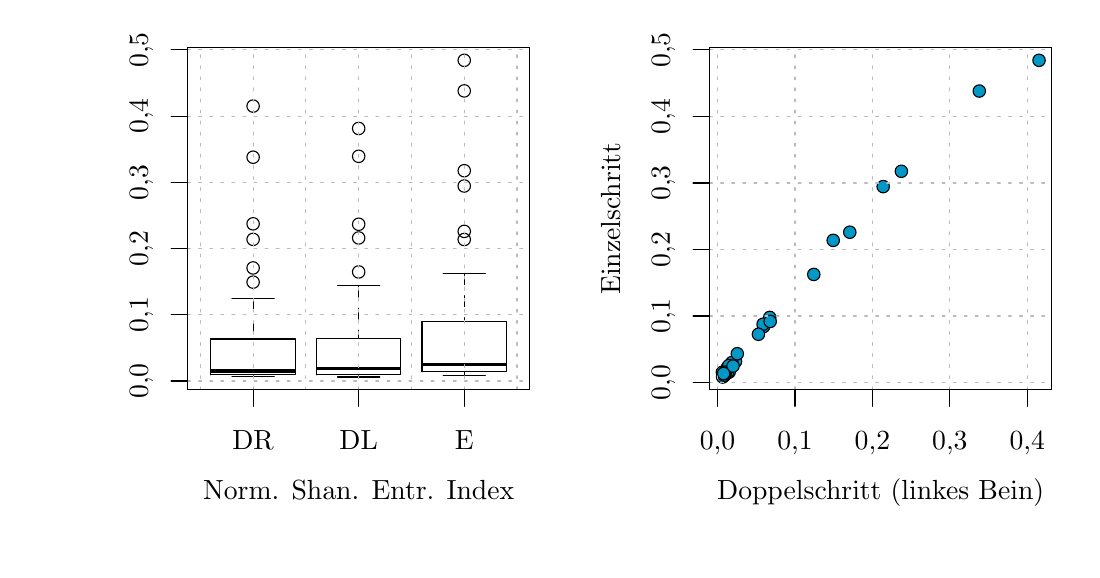
\begin{tikzpicture}[x=1pt,y=1pt]
\definecolor{fillColor}{RGB}{255,255,255}
\path[use as bounding box,fill=fillColor,fill opacity=0.00] (0,0) rectangle (377.25,188.62);
\begin{scope}
\path[clip] ( 57.82, 57.82) rectangle (181.40,181.40);
\definecolor{drawColor}{RGB}{0,0,0}

\path[draw=drawColor,line width= 1.2pt,line join=round] ( 66.21, 64.53) -- ( 96.72, 64.53);

\path[draw=drawColor,line width= 0.4pt,dash pattern=on 4pt off 4pt ,line join=round,line cap=round] ( 81.46, 62.42) -- ( 81.46, 63.18);

\path[draw=drawColor,line width= 0.4pt,dash pattern=on 4pt off 4pt ,line join=round,line cap=round] ( 81.46, 90.67) -- ( 81.46, 76.12);

\path[draw=drawColor,line width= 0.4pt,line join=round,line cap=round] ( 73.84, 62.42) -- ( 89.09, 62.42);

\path[draw=drawColor,line width= 0.4pt,line join=round,line cap=round] ( 73.84, 90.67) -- ( 89.09, 90.67);

\path[draw=drawColor,line width= 0.4pt,line join=round,line cap=round] ( 66.21, 63.18) --
	( 96.72, 63.18) --
	( 96.72, 76.12) --
	( 66.21, 76.12) --
	( 66.21, 63.18);

\path[draw=drawColor,line width= 0.4pt,line join=round,line cap=round] ( 81.46,101.80) circle (  2.25);

\path[draw=drawColor,line width= 0.4pt,line join=round,line cap=round] ( 81.46, 96.67) circle (  2.25);

\path[draw=drawColor,line width= 0.4pt,line join=round,line cap=round] ( 81.46,112.12) circle (  2.25);

\path[draw=drawColor,line width= 0.4pt,line join=round,line cap=round] ( 81.46,141.81) circle (  2.25);

\path[draw=drawColor,line width= 0.4pt,line join=round,line cap=round] ( 81.46,160.28) circle (  2.25);

\path[draw=drawColor,line width= 0.4pt,line join=round,line cap=round] ( 81.46,117.74) circle (  2.25);

\path[draw=drawColor,line width= 1.2pt,line join=round] (104.35, 65.35) -- (134.86, 65.35);

\path[draw=drawColor,line width= 0.4pt,dash pattern=on 4pt off 4pt ,line join=round,line cap=round] (119.61, 62.39) -- (119.61, 63.14);

\path[draw=drawColor,line width= 0.4pt,dash pattern=on 4pt off 4pt ,line join=round,line cap=round] (119.61, 95.30) -- (119.61, 76.40);

\path[draw=drawColor,line width= 0.4pt,line join=round,line cap=round] (111.98, 62.39) -- (127.24, 62.39);

\path[draw=drawColor,line width= 0.4pt,line join=round,line cap=round] (111.98, 95.30) -- (127.24, 95.30);

\path[draw=drawColor,line width= 0.4pt,line join=round,line cap=round] (104.35, 63.14) --
	(134.86, 63.14) --
	(134.86, 76.40) --
	(104.35, 76.40) --
	(104.35, 63.14);

\path[draw=drawColor,line width= 0.4pt,line join=round,line cap=round] (119.61,100.35) circle (  2.25);

\path[draw=drawColor,line width= 0.4pt,line join=round,line cap=round] (119.61,112.64) circle (  2.25);

\path[draw=drawColor,line width= 0.4pt,line join=round,line cap=round] (119.61,142.14) circle (  2.25);

\path[draw=drawColor,line width= 0.4pt,line join=round,line cap=round] (119.61,152.20) circle (  2.25);

\path[draw=drawColor,line width= 0.4pt,line join=round,line cap=round] (119.61,117.58) circle (  2.25);

\path[draw=drawColor,line width= 1.2pt,line join=round] (142.49, 66.86) -- (173.01, 66.86);

\path[draw=drawColor,line width= 0.4pt,dash pattern=on 4pt off 4pt ,line join=round,line cap=round] (157.75, 62.95) -- (157.75, 64.28);

\path[draw=drawColor,line width= 0.4pt,dash pattern=on 4pt off 4pt ,line join=round,line cap=round] (157.75, 99.82) -- (157.75, 82.43);

\path[draw=drawColor,line width= 0.4pt,line join=round,line cap=round] (150.12, 62.95) -- (165.38, 62.95);

\path[draw=drawColor,line width= 0.4pt,line join=round,line cap=round] (150.12, 99.82) -- (165.38, 99.82);

\path[draw=drawColor,line width= 0.4pt,line join=round,line cap=round] (142.49, 64.28) --
	(173.01, 64.28) --
	(173.01, 82.43) --
	(142.49, 82.43) --
	(142.49, 64.28);

\path[draw=drawColor,line width= 0.4pt,line join=round,line cap=round] (157.75,115.01) circle (  2.25);

\path[draw=drawColor,line width= 0.4pt,line join=round,line cap=round] (157.75,112.08) circle (  2.25);

\path[draw=drawColor,line width= 0.4pt,line join=round,line cap=round] (157.75,131.41) circle (  2.25);

\path[draw=drawColor,line width= 0.4pt,line join=round,line cap=round] (157.75,165.77) circle (  2.25);

\path[draw=drawColor,line width= 0.4pt,line join=round,line cap=round] (157.75,176.82) circle (  2.25);

\path[draw=drawColor,line width= 0.4pt,line join=round,line cap=round] (157.75,136.93) circle (  2.25);
\end{scope}
\begin{scope}
\path[clip] (  0.00,  0.00) rectangle (377.25,188.62);
\definecolor{drawColor}{RGB}{0,0,0}

\path[draw=drawColor,line width= 0.4pt,line join=round,line cap=round] ( 81.46, 57.82) -- (157.75, 57.82);

\path[draw=drawColor,line width= 0.4pt,line join=round,line cap=round] ( 81.46, 57.82) -- ( 81.46, 51.82);

\path[draw=drawColor,line width= 0.4pt,line join=round,line cap=round] (119.61, 57.82) -- (119.61, 51.82);

\path[draw=drawColor,line width= 0.4pt,line join=round,line cap=round] (157.75, 57.82) -- (157.75, 51.82);

\node[text=drawColor,anchor=base,inner sep=0pt, outer sep=0pt, scale=  1.00] at ( 81.46, 36.22) {DR};

\node[text=drawColor,anchor=base,inner sep=0pt, outer sep=0pt, scale=  1.00] at (119.61, 36.22) {DL};

\node[text=drawColor,anchor=base,inner sep=0pt, outer sep=0pt, scale=  1.00] at (157.75, 36.22) {E};

\path[draw=drawColor,line width= 0.4pt,line join=round,line cap=round] ( 57.82, 60.94) -- ( 57.82,180.58);

\path[draw=drawColor,line width= 0.4pt,line join=round,line cap=round] ( 57.82, 60.94) -- ( 51.82, 60.94);

\path[draw=drawColor,line width= 0.4pt,line join=round,line cap=round] ( 57.82, 84.87) -- ( 51.82, 84.87);

\path[draw=drawColor,line width= 0.4pt,line join=round,line cap=round] ( 57.82,108.80) -- ( 51.82,108.80);

\path[draw=drawColor,line width= 0.4pt,line join=round,line cap=round] ( 57.82,132.72) -- ( 51.82,132.72);

\path[draw=drawColor,line width= 0.4pt,line join=round,line cap=round] ( 57.82,156.65) -- ( 51.82,156.65);

\path[draw=drawColor,line width= 0.4pt,line join=round,line cap=round] ( 57.82,180.58) -- ( 51.82,180.58);

\node[text=drawColor,rotate= 90.00,anchor=base,inner sep=0pt, outer sep=0pt, scale=  1.00] at ( 43.42, 60.94) {0,0};

\node[text=drawColor,rotate= 90.00,anchor=base,inner sep=0pt, outer sep=0pt, scale=  1.00] at ( 43.42, 84.87) {0,1};

\node[text=drawColor,rotate= 90.00,anchor=base,inner sep=0pt, outer sep=0pt, scale=  1.00] at ( 43.42,108.80) {0,2};

\node[text=drawColor,rotate= 90.00,anchor=base,inner sep=0pt, outer sep=0pt, scale=  1.00] at ( 43.42,132.72) {0,3};

\node[text=drawColor,rotate= 90.00,anchor=base,inner sep=0pt, outer sep=0pt, scale=  1.00] at ( 43.42,156.65) {0,4};

\node[text=drawColor,rotate= 90.00,anchor=base,inner sep=0pt, outer sep=0pt, scale=  1.00] at ( 43.42,180.58) {0,5};
\end{scope}
\begin{scope}
\path[clip] (  0.00,  0.00) rectangle (188.62,188.62);
\definecolor{drawColor}{RGB}{0,0,0}

\node[text=drawColor,anchor=base,inner sep=0pt, outer sep=0pt, scale=  1.00] at (119.61, 18.22) {Norm. Shan. Entr. Index};
\end{scope}
\begin{scope}
\path[clip] (  0.00,  0.00) rectangle (377.25,188.62);
\definecolor{drawColor}{RGB}{0,0,0}

\path[draw=drawColor,line width= 0.4pt,line join=round,line cap=round] ( 57.82, 57.82) --
	(181.40, 57.82) --
	(181.40,181.40) --
	( 57.82,181.40) --
	( 57.82, 57.82);
\end{scope}
\begin{scope}
\path[clip] ( 57.82, 57.82) rectangle (181.40,181.40);
\definecolor{drawColor}{RGB}{186,187,194}

\path[draw=drawColor,line width= 0.4pt,dash pattern=on 1pt off 3pt ,line join=round,line cap=round] ( 62.39, 57.82) -- ( 62.39,181.40);

\path[draw=drawColor,line width= 0.4pt,dash pattern=on 1pt off 3pt ,line join=round,line cap=round] ( 81.46, 57.82) -- ( 81.46,181.40);

\path[draw=drawColor,line width= 0.4pt,dash pattern=on 1pt off 3pt ,line join=round,line cap=round] (100.54, 57.82) -- (100.54,181.40);

\path[draw=drawColor,line width= 0.4pt,dash pattern=on 1pt off 3pt ,line join=round,line cap=round] (119.61, 57.82) -- (119.61,181.40);

\path[draw=drawColor,line width= 0.4pt,dash pattern=on 1pt off 3pt ,line join=round,line cap=round] (138.68, 57.82) -- (138.68,181.40);

\path[draw=drawColor,line width= 0.4pt,dash pattern=on 1pt off 3pt ,line join=round,line cap=round] (157.75, 57.82) -- (157.75,181.40);

\path[draw=drawColor,line width= 0.4pt,dash pattern=on 1pt off 3pt ,line join=round,line cap=round] (176.82, 57.82) -- (176.82,181.40);

\path[draw=drawColor,line width= 0.4pt,dash pattern=on 1pt off 3pt ,line join=round,line cap=round] ( 57.82, 60.94) -- (181.40, 60.94);

\path[draw=drawColor,line width= 0.4pt,dash pattern=on 1pt off 3pt ,line join=round,line cap=round] ( 57.82, 84.87) -- (181.40, 84.87);

\path[draw=drawColor,line width= 0.4pt,dash pattern=on 1pt off 3pt ,line join=round,line cap=round] ( 57.82,108.80) -- (181.40,108.80);

\path[draw=drawColor,line width= 0.4pt,dash pattern=on 1pt off 3pt ,line join=round,line cap=round] ( 57.82,132.72) -- (181.40,132.72);

\path[draw=drawColor,line width= 0.4pt,dash pattern=on 1pt off 3pt ,line join=round,line cap=round] ( 57.82,156.65) -- (181.40,156.65);

\path[draw=drawColor,line width= 0.4pt,dash pattern=on 1pt off 3pt ,line join=round,line cap=round] ( 57.82,180.58) -- (181.40,180.58);
\end{scope}
\begin{scope}
\path[clip] (  0.00,  0.00) rectangle (377.25,188.62);
\definecolor{drawColor}{RGB}{0,0,0}

\path[draw=drawColor,line width= 0.4pt,line join=round,line cap=round] ( 57.82, 57.82) --
	(181.40, 57.82) --
	(181.40,181.40) --
	( 57.82,181.40) --
	( 57.82, 57.82);
\end{scope}
\begin{scope}
\path[clip] (246.44, 57.82) rectangle (370.02,181.40);
\definecolor{drawColor}{RGB}{0,0,0}
\definecolor{fillColor}{RGB}{0,152,199}

\path[draw=drawColor,line width= 0.4pt,line join=round,line cap=round,fill=fillColor] (251.95, 63.42) circle (  2.25);

\path[draw=drawColor,line width= 0.4pt,line join=round,line cap=round,fill=fillColor] (297.07,114.71) circle (  2.25);

\path[draw=drawColor,line width= 0.4pt,line join=round,line cap=round,fill=fillColor] (252.61, 64.42) circle (  2.25);

\path[draw=drawColor,line width= 0.4pt,line join=round,line cap=round,fill=fillColor] (253.49, 64.20) circle (  2.25);

\path[draw=drawColor,line width= 0.4pt,line join=round,line cap=round,fill=fillColor] (255.77, 67.97) circle (  2.25);

\path[draw=drawColor,line width= 0.4pt,line join=round,line cap=round,fill=fillColor] (268.14, 83.92) circle (  2.25);

\path[draw=drawColor,line width= 0.4pt,line join=round,line cap=round,fill=fillColor] (291.07,111.76) circle (  2.25);

\path[draw=drawColor,line width= 0.4pt,line join=round,line cap=round,fill=fillColor] (284.06, 99.45) circle (  2.25);

\path[draw=drawColor,line width= 0.4pt,line join=round,line cap=round,fill=fillColor] (251.23, 62.88) circle (  2.25);

\path[draw=drawColor,line width= 0.4pt,line join=round,line cap=round,fill=fillColor] (251.59, 62.77) circle (  2.25);

\path[draw=drawColor,line width= 0.4pt,line join=round,line cap=round,fill=fillColor] (309.14,131.19) circle (  2.25);

\path[draw=drawColor,line width= 0.4pt,line join=round,line cap=round,fill=fillColor] (265.94, 80.62) circle (  2.25);

\path[draw=drawColor,line width= 0.4pt,line join=round,line cap=round,fill=fillColor] (265.75, 81.47) circle (  2.25);

\path[draw=drawColor,line width= 0.4pt,line join=round,line cap=round,fill=fillColor] (268.30, 82.47) circle (  2.25);

\path[draw=drawColor,line width= 0.4pt,line join=round,line cap=round,fill=fillColor] (252.57, 64.58) circle (  2.25);

\path[draw=drawColor,line width= 0.4pt,line join=round,line cap=round,fill=fillColor] (264.06, 77.83) circle (  2.25);

\path[draw=drawColor,line width= 0.4pt,line join=round,line cap=round,fill=fillColor] (251.40, 63.20) circle (  2.25);

\path[draw=drawColor,line width= 0.4pt,line join=round,line cap=round,fill=fillColor] (254.48, 67.17) circle (  2.25);

\path[draw=drawColor,line width= 0.4pt,line join=round,line cap=round,fill=fillColor] (252.80, 63.85) circle (  2.25);

\path[draw=drawColor,line width= 0.4pt,line join=round,line cap=round,fill=fillColor] (343.86,165.72) circle (  2.25);

\path[draw=drawColor,line width= 0.4pt,line join=round,line cap=round,fill=fillColor] (251.13, 62.39) circle (  2.25);

\path[draw=drawColor,line width= 0.4pt,line join=round,line cap=round,fill=fillColor] (251.87, 63.83) circle (  2.25);

\path[draw=drawColor,line width= 0.4pt,line join=round,line cap=round,fill=fillColor] (365.45,176.82) circle (  2.25);

\path[draw=drawColor,line width= 0.4pt,line join=round,line cap=round,fill=fillColor] (254.42, 67.58) circle (  2.25);

\path[draw=drawColor,line width= 0.4pt,line join=round,line cap=round,fill=fillColor] (315.71,136.73) circle (  2.25);

\path[draw=drawColor,line width= 0.4pt,line join=round,line cap=round,fill=fillColor] (251.98, 63.17) circle (  2.25);

\path[draw=drawColor,line width= 0.4pt,line join=round,line cap=round,fill=fillColor] (251.02, 64.11) circle (  2.25);

\path[draw=drawColor,line width= 0.4pt,line join=round,line cap=round,fill=fillColor] (252.87, 65.82) circle (  2.25);

\path[draw=drawColor,line width= 0.4pt,line join=round,line cap=round,fill=fillColor] (253.38, 66.54) circle (  2.25);

\path[draw=drawColor,line width= 0.4pt,line join=round,line cap=round,fill=fillColor] (252.09, 64.14) circle (  2.25);

\path[draw=drawColor,line width= 0.4pt,line join=round,line cap=round,fill=fillColor] (251.70, 63.04) circle (  2.25);

\path[draw=drawColor,line width= 0.4pt,line join=round,line cap=round,fill=fillColor] (251.77, 63.59) circle (  2.25);

\path[draw=drawColor,line width= 0.4pt,line join=round,line cap=round,fill=fillColor] (254.88, 66.33) circle (  2.25);

\path[draw=drawColor,line width= 0.4pt,line join=round,line cap=round,fill=fillColor] (251.47, 63.63) circle (  2.25);

\path[draw=drawColor,line width= 0.4pt,line join=round,line cap=round,fill=fillColor] (256.42, 70.80) circle (  2.25);
\end{scope}
\begin{scope}
\path[clip] (  0.00,  0.00) rectangle (377.25,188.62);
\definecolor{drawColor}{RGB}{0,0,0}

\path[draw=drawColor,line width= 0.4pt,line join=round,line cap=round] (249.30, 57.82) -- (361.21, 57.82);

\path[draw=drawColor,line width= 0.4pt,line join=round,line cap=round] (249.30, 57.82) -- (249.30, 51.82);

\path[draw=drawColor,line width= 0.4pt,line join=round,line cap=round] (277.27, 57.82) -- (277.27, 51.82);

\path[draw=drawColor,line width= 0.4pt,line join=round,line cap=round] (305.25, 57.82) -- (305.25, 51.82);

\path[draw=drawColor,line width= 0.4pt,line join=round,line cap=round] (333.23, 57.82) -- (333.23, 51.82);

\path[draw=drawColor,line width= 0.4pt,line join=round,line cap=round] (361.21, 57.82) -- (361.21, 51.82);

\node[text=drawColor,anchor=base,inner sep=0pt, outer sep=0pt, scale=  1.00] at (249.30, 36.22) {0,0};

\node[text=drawColor,anchor=base,inner sep=0pt, outer sep=0pt, scale=  1.00] at (277.27, 36.22) {0,1};

\node[text=drawColor,anchor=base,inner sep=0pt, outer sep=0pt, scale=  1.00] at (305.25, 36.22) {0,2};

\node[text=drawColor,anchor=base,inner sep=0pt, outer sep=0pt, scale=  1.00] at (333.23, 36.22) {0,3};

\node[text=drawColor,anchor=base,inner sep=0pt, outer sep=0pt, scale=  1.00] at (361.21, 36.22) {0,4};

\path[draw=drawColor,line width= 0.4pt,line join=round,line cap=round] (246.44, 60.38) -- (246.44,180.60);

\path[draw=drawColor,line width= 0.4pt,line join=round,line cap=round] (246.44, 60.38) -- (240.44, 60.38);

\path[draw=drawColor,line width= 0.4pt,line join=round,line cap=round] (246.44, 84.42) -- (240.44, 84.42);

\path[draw=drawColor,line width= 0.4pt,line join=round,line cap=round] (246.44,108.46) -- (240.44,108.46);

\path[draw=drawColor,line width= 0.4pt,line join=round,line cap=round] (246.44,132.51) -- (240.44,132.51);

\path[draw=drawColor,line width= 0.4pt,line join=round,line cap=round] (246.44,156.55) -- (240.44,156.55);

\path[draw=drawColor,line width= 0.4pt,line join=round,line cap=round] (246.44,180.60) -- (240.44,180.60);

\node[text=drawColor,rotate= 90.00,anchor=base,inner sep=0pt, outer sep=0pt, scale=  1.00] at (232.04, 60.38) {0,0};

\node[text=drawColor,rotate= 90.00,anchor=base,inner sep=0pt, outer sep=0pt, scale=  1.00] at (232.04, 84.42) {0,1};

\node[text=drawColor,rotate= 90.00,anchor=base,inner sep=0pt, outer sep=0pt, scale=  1.00] at (232.04,108.46) {0,2};

\node[text=drawColor,rotate= 90.00,anchor=base,inner sep=0pt, outer sep=0pt, scale=  1.00] at (232.04,132.51) {0,3};

\node[text=drawColor,rotate= 90.00,anchor=base,inner sep=0pt, outer sep=0pt, scale=  1.00] at (232.04,156.55) {0,4};

\node[text=drawColor,rotate= 90.00,anchor=base,inner sep=0pt, outer sep=0pt, scale=  1.00] at (232.04,180.60) {0,5};

\path[draw=drawColor,line width= 0.4pt,line join=round,line cap=round] (246.44, 57.82) --
	(370.02, 57.82) --
	(370.02,181.40) --
	(246.44,181.40) --
	(246.44, 57.82);
\end{scope}
\begin{scope}
\path[clip] (188.62,  0.00) rectangle (377.25,188.62);
\definecolor{drawColor}{RGB}{0,0,0}

\node[text=drawColor,anchor=base,inner sep=0pt, outer sep=0pt, scale=  1.00] at (308.23, 18.22) {Doppelschritt (linkes Bein)};

\node[text=drawColor,rotate= 90.00,anchor=base,inner sep=0pt, outer sep=0pt, scale=  1.00] at (214.04,119.61) {Einzelschritt};
\end{scope}
\begin{scope}
\path[clip] (246.44, 57.82) rectangle (370.02,181.40);
\definecolor{drawColor}{RGB}{186,187,194}

\path[draw=drawColor,line width= 0.4pt,dash pattern=on 1pt off 3pt ,line join=round,line cap=round] (249.30, 57.82) -- (249.30,181.40);

\path[draw=drawColor,line width= 0.4pt,dash pattern=on 1pt off 3pt ,line join=round,line cap=round] (277.27, 57.82) -- (277.27,181.40);

\path[draw=drawColor,line width= 0.4pt,dash pattern=on 1pt off 3pt ,line join=round,line cap=round] (305.25, 57.82) -- (305.25,181.40);

\path[draw=drawColor,line width= 0.4pt,dash pattern=on 1pt off 3pt ,line join=round,line cap=round] (333.23, 57.82) -- (333.23,181.40);

\path[draw=drawColor,line width= 0.4pt,dash pattern=on 1pt off 3pt ,line join=round,line cap=round] (361.21, 57.82) -- (361.21,181.40);

\path[draw=drawColor,line width= 0.4pt,dash pattern=on 1pt off 3pt ,line join=round,line cap=round] (246.44, 60.38) -- (370.02, 60.38);

\path[draw=drawColor,line width= 0.4pt,dash pattern=on 1pt off 3pt ,line join=round,line cap=round] (246.44, 84.42) -- (370.02, 84.42);

\path[draw=drawColor,line width= 0.4pt,dash pattern=on 1pt off 3pt ,line join=round,line cap=round] (246.44,108.46) -- (370.02,108.46);

\path[draw=drawColor,line width= 0.4pt,dash pattern=on 1pt off 3pt ,line join=round,line cap=round] (246.44,132.51) -- (370.02,132.51);

\path[draw=drawColor,line width= 0.4pt,dash pattern=on 1pt off 3pt ,line join=round,line cap=round] (246.44,156.55) -- (370.02,156.55);

\path[draw=drawColor,line width= 0.4pt,dash pattern=on 1pt off 3pt ,line join=round,line cap=round] (246.44,180.60) -- (370.02,180.60);
\end{scope}
\begin{scope}
\path[clip] (  0.00,  0.00) rectangle (377.25,188.62);
\definecolor{drawColor}{RGB}{0,0,0}

\path[draw=drawColor,line width= 0.4pt,line join=round,line cap=round] (246.44, 57.82) --
	(370.02, 57.82) --
	(370.02,181.40) --
	(246.44,181.40) --
	(246.44, 57.82);
\end{scope}
\end{tikzpicture}
 \caption[Kardio-lokomotorischen Phasensynchronation: Vergleich der Doppelschrittberechnung und Einzelschrittberechnung]{Kardio-lokomotorischen Phasensynchronation: Vergleich der Doppelschrittberechnung und Einzelschrittberechnung: (rechts) Mittelwertvergleich; (links) Zusammenhang zwischen Doppelschrittberechnung ausgehend vom linken Bein und Einzelschrittberechnung. \emph{Anmerkung}: \\ \hspace{\textwidth}DL = Doppelschrittberechnung ausgehend vom linken Bein \\ \hspace{\textwidth}DR = Doppelschrittberechnung ausgehend vom rechten Bein \\ \hspace{\textwidth}E = Einzelschritt} \label{fig:index_vergleich} 
\end{figure}

% subsection operationalisierung_und_gewonnene_daten (end)
% section flow_und_laufen_interindividuell (end)
